\chapter{Qualitätsszenarien}
\label{ch:Qualitaetsszenarien}

\section{Verfügbarkeits-Szenario}
\begin{figure}[tbh]
  \centering
  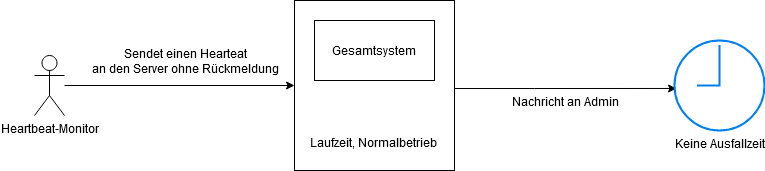
\includegraphics[width=0.7\textwidth]{Graphics/Verfuegbarkeit.png}
  \caption{Verfügbarkeits-Szenario}
  \label{fig:Qualitaet1}
\end{figure}

Verfügbarkeits-Szenario\\
Source of Stimulus: Heartbeat Monitor\\
Stimulus: Sendet einen Heartbeat an den Server ohne Rückmeldung\\
Environment: Laufzeit, Normalbetrieb\\
Component: Gesamtsystem\\
Response: Nachricht an Admin\\
Response Measure: Keine Ausfallzeit\\

Heartbeat an eine Serverkomponente geschickt.  Dadurch haben wir ein Verteiltes System


\section{Sicherheits-Szenario}
\begin{figure}[tbh]
  \centering
  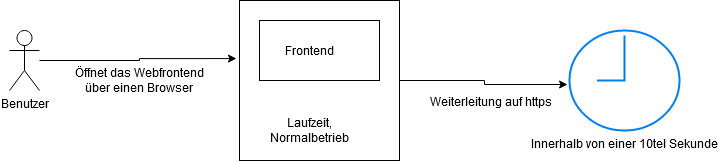
\includegraphics[width=0.7\textwidth]{Graphics/Sicherheit.png}
  \caption{Sicherheit-Szenario}
  \label{fig:Qualitaet2}
\end{figure}


Sicherheits-Szenario\\
Source of Stimulus: Benutzer\\
Stimulus: Öffnet das Webfrontend über einen Browser über http\\
Environment: Laufzeit, Normalbetrieb\\
Component: Frontend\\
Response: Weiterleitung auf https\\
Response Measure: Daten sind verschlüsselt\\



\section{Nutzbarkeits-Szenario}
\begin{figure}[tbh]
  \centering
  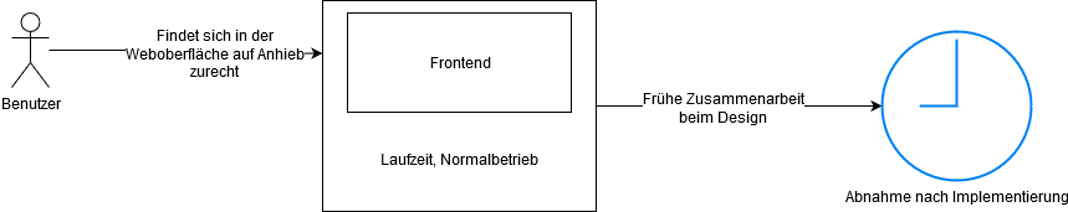
\includegraphics[width=0.7\textwidth]{Graphics/Nutzbarkeit.png}
  \caption{Nutzbarkeit-Szenario}
  \label{fig:Qualitaet3}
\end{figure}



Nutzbarkeits-Szenario
Source of Stimulus: Benutzer\\
Stimulus: Öffnet das Webfrontend\\
Environment: Laufzeit, Normalbetrieb\\
Component: Frontend\\
Response: Öffnet das Tutorial / Hilfe-Meldung\\
Response Measure: Neue Nutzer haben einen guten Einstieg in der Software\\




\section{Erweiterbarkeits-Szenario}
\begin{figure}[tbh]
  \centering
  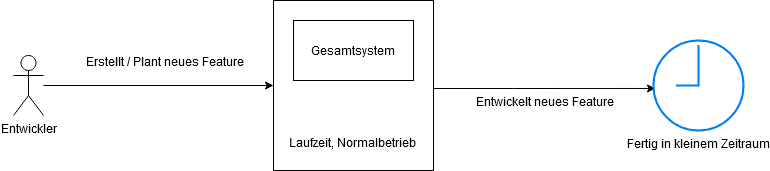
\includegraphics[width=0.7\textwidth]{Graphics/Erweiterbarkeit.png}
  \caption{Erweiterbarkeits-Szenario}
  \label{fig:Qualitaet3}
\end{figure}


Erweiterbarkeits-Szenario\\
Source of Stimulus: Entwickler\\
Stimulus: Erstellt / Plant neues Feature\\
Environment: Laufzeit, Normalbetrieb\\
Component: Gesamtsystem\\
Response: Implementierung ohne negativen Sideeffects\\
Response Measure: Implementierung innerhalb einer Woche \\


\section{Portierbarkeit-Szenario}
\begin{figure}[tbh]
  \centering
  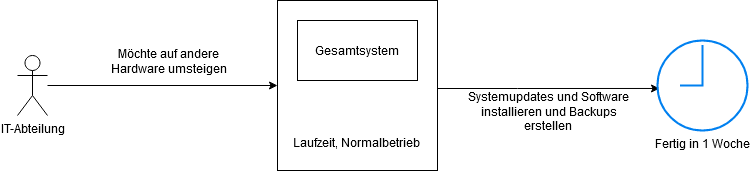
\includegraphics[width=0.7\textwidth]{Graphics/Portierbarkeit.png}
  \caption{Portierbarkeit-Szenario}
  \label{fig:Qualitaet4}
\end{figure}



Portierbarkeits-Szenario\\
Source of Stimulus: IT-Abteilung\\
Stimulus: Möchte auf andere Hardware umsteigen\\
Environment: Laufzeit, Normalbetrieb\\
Component: Gesamtsystem\\
Response: Systemupdates und Software installieren und Backups erstellen \\
Response Measure: Fertig in 1 Woche\\



\section{Effizienz-Szenario}
\begin{figure}[tbh]
  \centering
  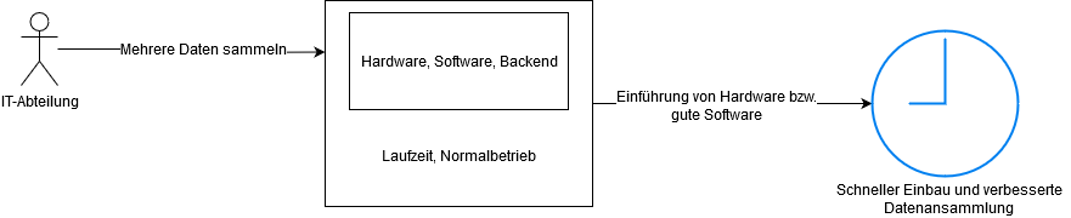
\includegraphics[width=0.7\textwidth]{Graphics/Effizienz.png}
  \caption{Effizienz-Szenario}
  \label{fig:Qualitaet5}
\end{figure}



Effizienz-Szenario\\
Source of Stimulus: Entwickler\\
Stimulus: Mehrere Daten sammeln\\
Environment:Laufzeit, Normalbetrieb\\
Component: Hardware, Software, Backend\\
Response: Einführung von Hardware, bzw. gute Software um Datenpunkte zu sammeln\\
Response Measure: Schneller Einbau und verbesserte Datensammlung\\



\section{Hardware-Szenario}
\begin{figure}[tbh]
  \centering
  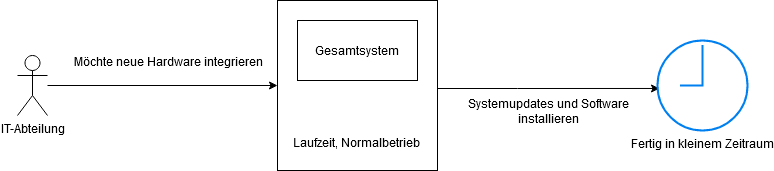
\includegraphics[width=0.7\textwidth]{Graphics/Hardware.png}
  \caption{Hardware-Szenario}
  \label{fig:Qualitaet6}
\end{figure}


Hardware-Szenario\\
Source of Stimulus: IT-Abteilung\\
Stimulus: Möchte neue Hardware integrieren\\
Environment:Lautzeit, Normalbetrieb\\
Component: Gesamtsystem\\
Response: Systemupdates und Software installieren\\
Response Measure: Fertig in kleinen Zeitraum\\

